%% March 2018
%%%%%%%%%%%%%%%%%%%%%%%%%%%%%%%%%%%%%%%%%%%%%%%%%%%%%%%%%%%%%%%%%%%%%%%%%%%%
% AGUJournalTemplate.tex: this template file is for articles formatted with LaTeX
%
% This file includes commands and instructions
% given in the order necessary to produce a final output that will
% satisfy AGU requirements, including customized APA reference formatting.
%
% You may copy this file and give it your
% article name, and enter your text.
%
%%%%%%%%%%%%%%%%%%%%%%%%%%%%%%%%%%%%%%%%%%%%%%%%%%%%%%%%%%%%%%%%%%%%%%%%%%%%
% PLEASE DO NOT USE YOUR OWN MACROS
% DO NOT USE \newcommand, \renewcommand, or \def, etc.
%
% FOR FIGURES, DO NOT USE \psfrag or \subfigure.
% DO NOT USE \psfrag or \subfigure commands.
%%%%%%%%%%%%%%%%%%%%%%%%%%%%%%%%%%%%%%%%%%%%%%%%%%%%%%%%%%%%%%%%%%%%%%%%%%%%
%
% Step 1: Set the \documentclass
%
% There are two options for article format:
%
% PLEASE USE THE DRAFT OPTION TO SUBMIT YOUR PAPERS.
% The draft option produces double spaced output.
%

%% To submit your paper:
%\documentclass[draft,linenumbers]{agujournal2018}  %%%%%%%%%%switch this back for linenumbers
%\documentclass[draft]{agujournal2018}
%\usepackage{apacite}
%\usepackage{url} %this package should fix any errors with URLs in refs.

\documentclass[main.tex]{subfiles}


%%%%%%%
% \usepackage{trackchanges}
% uncomment the line above to use the TrackChanges package to mark revisions if needed.
% The trackchanges package adds five new LaTeX commands:
%
%  \note[editor]{The note}
%  \annote[editor]{Text to annotate}{The note}
%  \add[editor]{Text to add}
%  \remove[editor]{Text to remove}
%  \change[editor]{Text to remove}{Text to add}
%
% complete documentation is here: http://trackchanges.sourceforge.net/
%%%%%%%

%\draftfalse

% Now, type in the journal name: \journalname{<Journal Name>}

% ie, \journalname{Journal of Geophysical Research}
%% Choose from this list of Journals:
%
% JGR-Atmospheres
% JGR-Biogeosciences
% JGR-Earth Surface
% JGR-Oceans
% JGR-Planets
% JGR-Solid Earth
% JGR-Space Physics
% Global Biochemical Cycles
% Geophysical Research Letters
% Paleoceanography
% Radio Science
% Reviews of Geophysics
% Tectonics
% Space Weather
% Water Resource Research
% Geochemistry, Geophysics, Geosystems
% Journal of Advances in Modeling Earth Systems (JAMES)
% Earth's Future
% Earth and Space Science
% Geohealth
%

%\journalname{Journal of Geophysical Research}


\begin{document}

%% ------------------------------------------------------------------------ %%
%  Title
%
% (A title should be specific, informative, and brief. Use
% abbreviations only if they are defined in the abstract. Titles that
% start with general keywords then specific terms are optimized in
% searches)
%
%% ------------------------------------------------------------------------ %%

% Example: \title{This is a test title}

%\title{A Low Cost Fiber-Optic Displacement Sensor Designed For Use at High Pressure}

%% ------------------------------------------------------------------------ %%
%
%  AUTHORS AND AFFILIATIONS
%
%% ------------------------------------------------------------------------ %%

% Authors are individuals who have significantly contributed to the
% research and preparation of the article. Group authors are allowed, if
% each author in the group is separately identified in an appendix.)

% List authors by first name or initial followed by last name and
% separated by commas. Use \affil{} to number affiliations, and
% \thanks{} for author notes.
% Additional author notes should be indicated with \thanks{} (for
% example, for current addresses).

% Example: \authors{A. B. Author\affil{1}\thanks{Current address, Antartica}, B. C. Author\affil{2,3}, and D. E.
% Author\affil{3,4}\thanks{Also funded by Monsanto.}

\authors{Eric Burdette and Greg Hirth}


%\affiliation{1}{Brown University}
% \affiliation{2}{Second Affiliation}
% \affiliation{3}{Third Affiliation}
% \affiliation{4}{Fourth Affiliation}

\affiliation{1}{Department of Earth, Environmental and Planetary Sciences, Brown University, Providence, RI, USA}
%(repeat as many times as is necessary)

%% Corresponding Author:
% Corresponding author mailing address and e-mail address:

% (include name and email addresses of the corresponding author.  More
% than one corresponding author is allowed in this LaTeX file and for
% publication; but only one corresponding author is allowed in our
% editorial system.)

% Example: \correspondingauthor{First and Last Name}{email@address.edu}

%\correspondingauthor{Eric Burdette}{eric\_burdette@brown.edu}

%% Keypoints, final entry on title page.

% Example:
% \begin{keypoints}
% \item	List up to three key points (at least one is required)
% \item	Key Points summarize the main points and conclusions of the article
% \item	Each must be 100 characters or less with no special characters or punctuation
% \end{keypoints}

%  List up to three key points (at least one is required)
%  Key Points summarize the main points and conclusions of the article
%  Each must be 100 characters or less with no special characters or punctuation

\begin{keypoints}
\item Seal friction limits stress resolution in high pressure deformation experiments without synchrotron imaging. Internal load measurement resolves this limitation.
\item The cell operates by measuring displacement of an elastic cavity. It is compact and can survive temperatures up to 700°C
\item Implementation is simple, requiring at minimum a PC, 96kHz sound card, telecom modulated DFB laser, and a photodiode.
\end{keypoints}

%% ------------------------------------------------------------------------ %%
%
%  ABSTRACT
%
% A good abstract will begin with a short description of the problem
% being addressed, briefly describe the new data or analyses, then
% briefly states the main conclusion(s) and how they are supported and
% uncertainties.
%% ------------------------------------------------------------------------ %%

%% \begin{abstract} starts the second page

\doublespacing


\begin{abstract}
Deforming rocks presents a particularly challenging test environment. Not only are required temperatures often above 300°C, but pressures above 200 MPa are commonly required to replicate conditions in the earth. The machines (Paterson-type, Griggs-type, D-DIA, Oxford Creep Rig, etc.) designed to apply these pressures and temperatures require measurement compromises and exotic materials to accommodate common, reliable sensors. Each of these machines has a furnace which can reach 1200°C at its center, often inside a pressure vessel. Common sensors like LVDTs and strain gauges cannot survive this temperature and are placed either outside the pressure vessel, or far from the furnace with ceramic or steel connecting rods/pistons. This can introduce unacceptable error into measurements of low stresses and specimen deformation rates sometimes as low as 1 μm/day, especially when friction is included. These applications would benefit from inclusion of a simple, compact, low cost displacement sensor with resolution better than 1 μm, which is achievable using an interferometer constructed with standard telecom fiber optic components.
We have adapted designs for external cavity Fabry-Perot interferometer to build a high accuracy (0.1 MPa, 2 nm) displacement/load sensor using standard telecom fiber/lasers and a disposable sensing head. The total equipment cost is less than \$5000.  The design was tested inside a Griggs pressure vessel to measure loads at 700°C.  A benefit of using telecom equipment is very large bandwidth. Using an FPGA for digital signal processing, bandwidth can easily reach 100 kHz, measuring speeds up to 20 mm/s. A small modification of the light path allows a vibrometer to be constructed, unlocking significantly higher speed/bandwidth (10 MHz).

\end{abstract}

%% ------------------------------------------------------------------------ %%
%
%  TEXT
%
%% ------------------------------------------------------------------------ %%


\section{Introduction}
Fiber optics allow direct measurement of sub-nanometer distances at extreme conditions which would otherwise be inaccessible to mechanical sensors like LVDTs. They also have the advantages in electrical interference immunity and no required additional mass. However, they lack the simplicity, reliability, and familiarity of electrical and magnetic displacement sensors. As a result laser displacement sensors are typically only found in exotic equipment with unusually low temperature, high speed, or high precision. A familiar example is the reflected red diode laser and detector used to measure position of atomic force microscopes.

Deforming rocks presents a particularly challenging environment. Not only are required temperatures often above 300°C, but pressure above 200 MPa are commonly required to replicate conditions in the earth. The machines (Paterson-type, Griggs-type, D-DIA, Oxford Creep Rig, etc.) designed to apply these pressures and temperatures require measurement compromises and exotic materials to accommodate common, reliable sensors. Each of these machines has a furnace which can reach 1200°C at its center, often inside a pressure vessel. Common sensors like LVDTs and strain gauges cannot survive this temperature and are placed either outside the pressure vessel, or far from the furnace with ceramic or steel connecting rods/pistons. This can introduce unacceptable error into measurements of low stresses and specimen strain rates sometimes approaching $1 \mu$m/day, especially when friction is included. These applications would benefit from inclusion of a simple, compact, low cost displacement sensor with resolution better than $1 \mu$m, which is achievable using an interferometer constructed with standard telecom fiber optic components.

Mass production of diode lasers has driven down cost to the point that a fiber-coupled, temperature stabilized laser diode system can be purchased for \$2000, while telecom fiber and detection equipment can be purchased for less than \$1000. Modulation, demodulation, and processing of laser intensity can be driven with common PC sound card equipment, bringing total cost to less than \$5000.

Two interferometer types stand out for application to our displacement applications: Mach-Zender and Fabry-Perot. Designs for Mach-Zender interferometers are already common in free space laser-doppler vibrometers which could be fiber-coupled.  Fabry-Perot designs are also common for strain/pressure sensing, and commercial fiber-coupled versions can be purchased for \$25,000. We describe a simpler version using laser intensity modulation.

An external cavity Fabry-Perot interferometer modulates reflected/transmitted intensity due to mutual interference between standing waves established in a cavity with partially reflecting mirrors. The simple design which we use is outlined by \citet{nowakowski2016highly}. The equation for intensity returning from the cavity is:
\begin{equation}
    \frac{I_{refl}}{I_{inc}} = \frac{\left(1+R\right)^2}{2}\frac{1-\cos{\frac{4\pi}{\lambda}h}}{1+R^2-2R\cos{\frac{4\pi}{\lambda}h}}
\end{equation}
where I is incident and reflected intensity, R is reflectance of the cavity surfaces, h is cavity length, and $\lambda$ is laser wavelength. Note that intensity changes with both cavity length and wavelength on a period of half the incident wavelength.

\citet{nowakowski2016highly} use a tunable wavelength laser ($\pm25$ nm) to oscillate wavelength at frequency f, and recover the reflected direct cavity response slope at f, while also recovering the curvature of the cavity response at frequency 2f. These signals are 90 degrees out of phase, so they can be separately demodulated and fed into an arctangent function to recover the phase of the cavity response, which is directly related to half the incident wavelength \citep[See\ ][]{kirkendall2004overview}. Using a 1550 nm laser, 10 bit accuracy can measure a 1 nm cavity length change.

\begin{figure}
  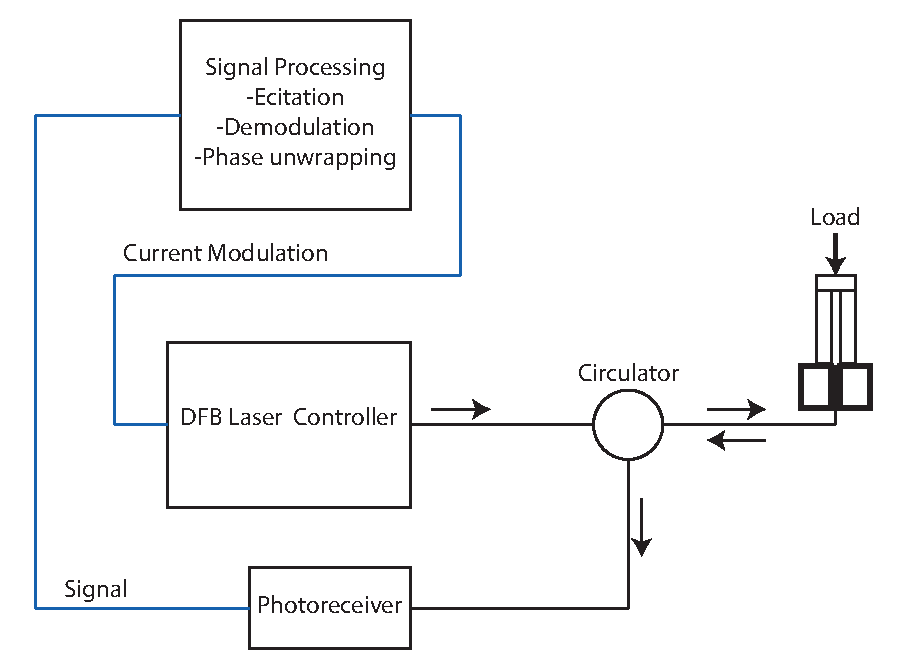
\includegraphics[width=\textwidth]{Figures/EFPI_diagram.pdf}
  \caption{Schematic of elements required for this EFPI system to measure load.}
  \label{fig:CH4_LaserSystemSchematic}
\end{figure}

\section{Sensor Design and Machine Integration}

    \subsection{Interferometer System}
        A schematic of the EFPI (External cavity Fabry-Perot Interferometer) implementation is presented in Figure \ref{fig:CH4_LaserSystemSchematic}. The system is comprised of a DFB laser controller (Koheron CTL200 with a QPhotonics qdfbld-1550-5), 2:1 FBT coupler, Fabry-Perot cavity (simplest form is a polished reflector and FC coupler terminated fiber), fiber coupled photodiode reciever (TTI TIA-950), and a digital-to analog/analog-to-digital converter on the same clock source with a signal processor (Digilent Eclypse Z7 FPGA or PC + sound card). A simple single frequency, current modulating laser is used instead of a tunable laser used by \citet{nowakowski2016highly}. The intensity and wavelength of the single-frequency laser changes with current. The wavelength-current coefficient is approximately 10 pm/mA, so the effective $\pm$25 mA modulation depth of the laser is enough to drive cavities greater than 5 mm long \citep{nowakowski2016highly}.

\begin{figure}
  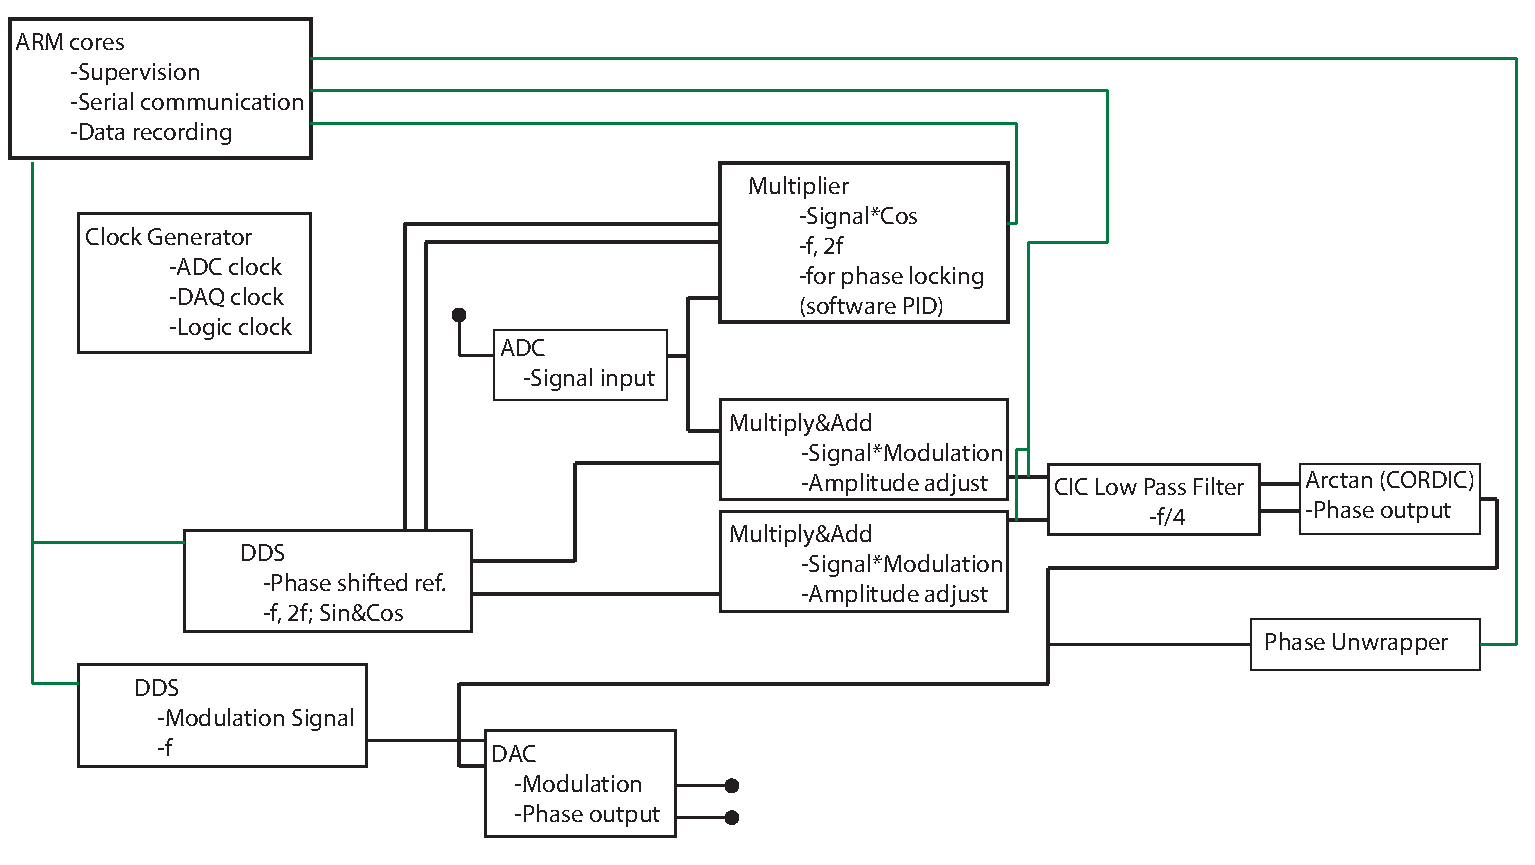
\includegraphics[width=\textwidth]{Figures/EFPI_DSP-FPGA_schematic.pdf}
  \caption{Schematic of the EFPI modulation and demodulation system implemented on a Digilent Eclypse Z7.}
  \label{fig:CH4_ProcessingSchematic}
\end{figure}
        
        Processing of the cavity length can be performed in realtime by a PC or FPGA with the scheme illustrated in Figure \ref{fig:CH4_ProcessingSchematic}. Maximum tracking speed at 6 kHz modulation frequency (for a PC sound card sampling at 96kHz) is 0.5 mm/s, while maximum tracking speed at 1.5 MHz modulation frequency is ???? mm/s. Bandwidth is limited by filtering to 3 kHz and 400 kHz respectively. 
        
        Because the amplitude of the 2f curvature produced by current/wavelength change is a secondary effect, its amplitude is always lower than that of the fundamental modulation frequency. This leads to a slightly oval-shaped path when the two components are plotted against each other which can be corrected at system startup.
        
    \subsection{Implementation to Measure Internal Axial Stress in a Griggs-Type Apparatus}
    
\begin{figure}
  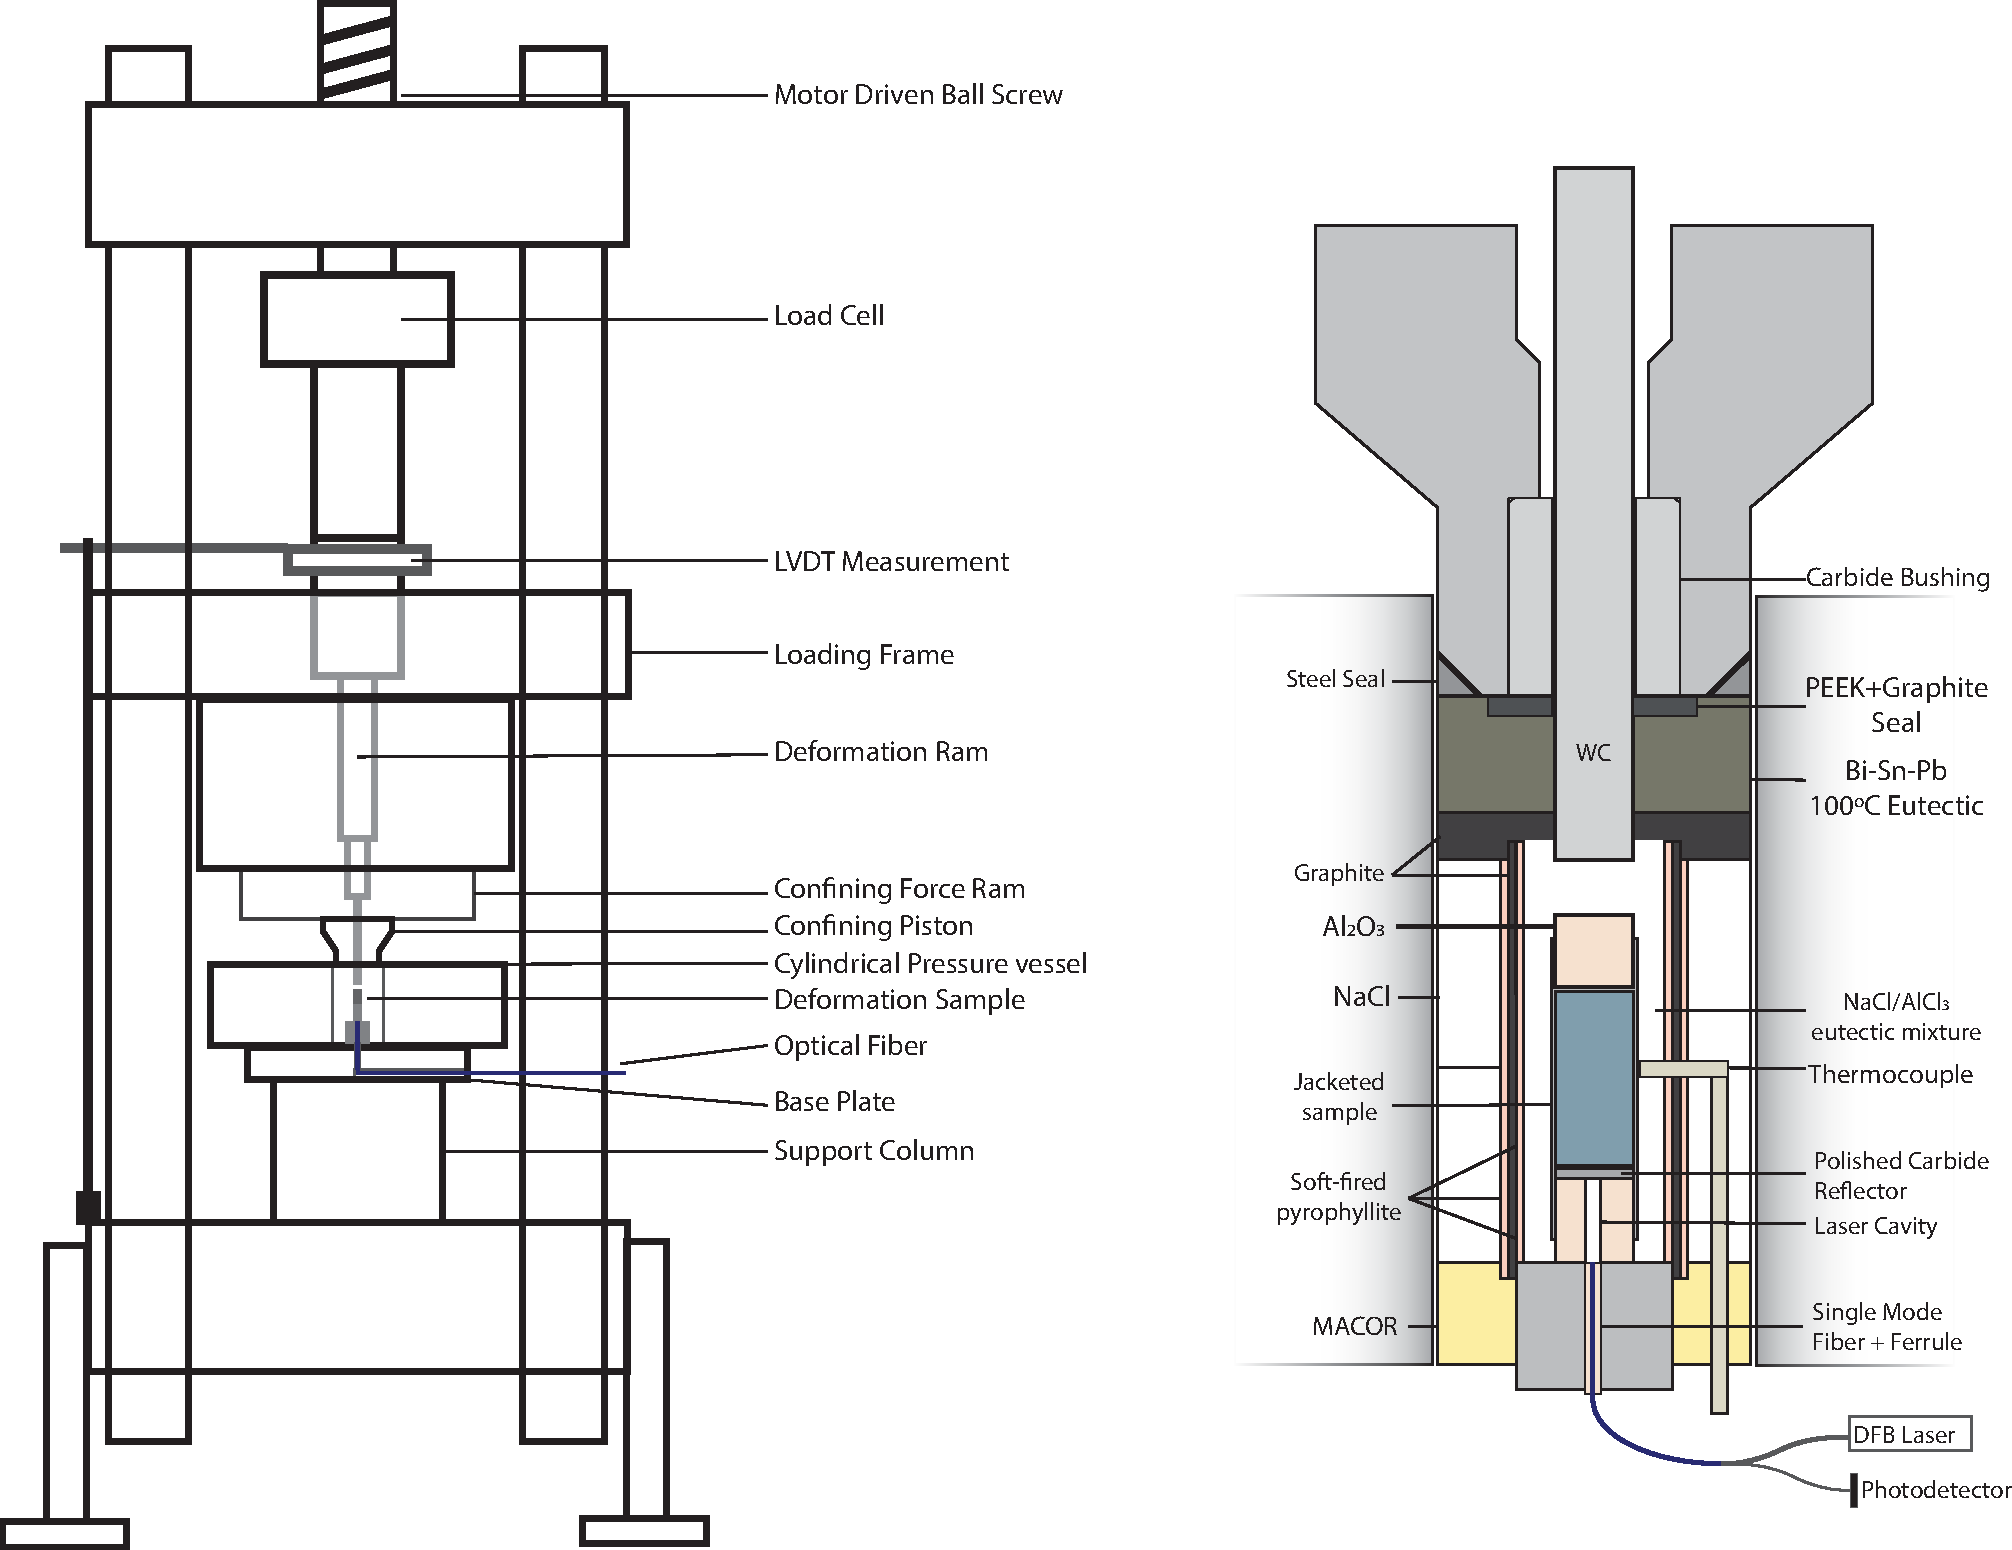
\includegraphics[width=\textwidth]{Figures/Fullrig1_WLaser.pdf}
  \caption{Schematic of implementation of the EFPI as a load cell in a Griggs-type high pressure deformation apparatus.}
  \label{fig:CH4_GriggsImplementation}
\end{figure}

        Figure \ref{fig:CH4_GriggsImplementation} shows how a cavity can be introduced into the loading column of a Griggs-type rock deformation apparatus. Fiber is fed up a hole in the central column and glued into the base carbide. A cavity (tube) sits on top of the base carbide, and a polished carbide reflector is placed below the sample to be deformed. A 10mm alumina tube with an elastic modulus of 400 GPa should change length by 25 nm for a 1 MPa stress change, which is well within the detection capabilities of the EFPI setup.
        
        A similar design was built by \citet{blacic1977wide} with excellent sensitivity. This design improves on their implementation by: improving immunity to pressure changes, improving immunity to vibration, and constructing the cavity from simple, inexpensive replaceable parts. The wide machined carbide pedestal of \citet{blacic1977wide} has axial area exposed to confining media which applies axial shortening force ~3x the axial deformation force, so small changes in pressure result in large cavity displacements that are indistinguishable from sample deformation loading. The cavity we implemented is the same diameter as the sample, so pressure changes can only affect its length through the Poisson effect. We improve noise immunity by using a terminated fiber glued directly underneath the cavity to avoid the external vibration influences (\citet{blacic1977wide}'s cavity was 14.6 cm including a significant amount of metal that changes size with total apparatus load/vibration and changes in room temperature). Finally, the fiber ferrule, alumina tube, and polished carbide are standard parts from materials suppliers (McMaster-Carr, Thorlabs), while the carbide is EDM drilled after purchase. After use, glue is burned out of the base carbide and ferrule at 400°C, and another is inserted and glued in for the next use.

\section{Results}

\begin{figure}
  \includegraphics[width=\textwidth]{Figures/W2534_75C.pdf}
  \caption{Plot of load and external displacement records from an experiment deforming a 360 grade brass sample.}
  \label{fig:CH4_Wax_LoadcellTest}
\end{figure}

    \subsection{Mechanical Results}
        For this testing, 1/4" cylinders of 360 grade brass were purchased from McMaster-Carr and deformed with the Griggs-type appratus inside a pressure vessel filled with melted paraffin wax at 150 MPa confining pressure. The lower portion of the loading column is jacketed in polyolefin to prevent wax from intruding in between column elements. A gap is left between the top piston and an externally connected piston so that the sample and lower column do not interact with the external piston until it is advanced after pressurization.
        
        Results from our traditional external load measurement and the new internal load cell are plotted against externally measured piston displacement (Figure \ref{fig:CH4_Wax_LoadcellTest}). When the externally connected piston is out of contact with the sample, internal load does not change regardless of which direction the piston is moving. While the piston is in contact with the column, deforming the sample, there is a static, direction dependent offset as would be expected for frictional hysteresis due to the seals.
        

\section{Conclusions}

    
    \begin{enumerate}
        \item We designed and tested an EFPI load sensor for high confining pressure deformation.
        \item Designs for the sensor are published here and can be replicated at low cost.
        \item Tests of pressure show the sensor has precision that meets or exceeds current requirements.
        \item The technology also can be used for high speed/precision displacement sensing during creep of brittle rocks.
    \end{enumerate}

%Text here ===>>>

\acknowledgments


%% ------------------------------------------------------------------------ %%
%% References and Citations

%\bibliography{Feb19_refs_2.bib}

\clearpage
\subfile{./EB_LaserLoadCell_SuppInfo.tex}

\clearpage

\singlespacing


\end{document}